 
\chapter{Desenvolvimento das arquiteturas propostas}
\label{cap5}


\section{Topologia da Rede}
\label{sec:topologia}

A topologia da rede seguiu o padrão proposto na Seção~\ref{cap3}.
%
O principal objetivo desta topologia é segregar as instâncias na camada de rede, evitando interferências do orquestrador de microsserviços que é utilizado na etapa de implantação, visto que a implantação dos clientes também é feita com um orquestrador de microsserviços para facilitar a execução dos experimentos.

A segregação em sub-redes é importante visto que, a fim de otimizar o transporte de dados entre os serviços, tais orquestradores trocam mensagens na rede utilizando memória quando a conexão é realizada para o próprio hospedeiro.
%
Segregando em sub-redes, o orquestrador é forçado a realizar a conexão com as instâncias externas utilizando a pilha completa dos protocolos \ac{tcp} e \ac{udp}, a qual são eventuais pontos de gargalo em tais arquiteturas.
%
Nesse sentido, espera-se que não exista troca de mensagens entre o cliente e serviço de jogo executando em memória.
%
Dessa forma, abre-se espaço para analisar eventuais gargalos na rede.

Para gerenciar as sub-redes da topologia, foi utilizado o gestor de sub-redes da Nuvem Tchê~\footnote{Nuvem Tche: \url{http://www.labp2d.joinville.udesc.br/}}, a qual é um serviço básico do sistema de gestor de nuvens computacionais OpenStack~\footnote{OpenStack: \url{https://www.openstack.org/}}.
%
Tal gestor acopla interfaces de rede virtuais a instâncias computacionais selecionadas, a fim de conecta-las a uma sub-rede virtualizada dentro do sistem OpenStack.

Utilizando o gestor do OpenStack, foram criadas 4 sub-redes a fim de isolar a rede do banco de dados, rede do serviço de jogo, rede dos clientes e rede do serviço de métricas.
%
Tal topologia utilizada nos experimentos com as arquiteturas Rudy, Salz e Willson podem ser visualizada na Figura~\ref{fig:topologia}.


\begin{figure}[htb!]
    \caption{Topologia da rede no gestor de redes do OpenStack.}
    \centering
    \begin{subfigure}{0.5\textwidth}
      \centering
      \includegraphics[width=.8\textwidth]{img/cap5/topology_graph.png}
      \caption{Grafo OpenStack do experimento.}
      \label{fig:topologia_a}
    \end{subfigure}%
    \begin{subfigure}{0.5\textwidth}
      \centering
      \includegraphics[width=.8\textwidth]{img/cap5/topology.png}
      \caption{Topologia da rede OpenStack.}
      \label{fig:topologia_b}
    \end{subfigure}
    \label{fig:topologia}

    Fonte: O próprio autor.
\end{figure}


A Figura~\ref{fig:topologia} mostra a disposição das instâncias em sub-redes exibindo-as como um grafo (Subfigura~\ref{fig:topologia_a}) e em forma de barramento (Subfigura~\ref{fig:topologia_b}).
%
A visualização em Grafo ajuda a compreender a disposição das instâncias computacionais e a conectividade entre cada instância do ambiente de experimentos.
%
Já a visualização em barramento exibe características técnicas como a faixa de \ac{ip} e nome das sub-redes.
%
Ambos os gráficos são complementares para informar as características básicas da interconexão das sub-redes.

A Figura~\ref{fig:topologia} também exibe 8 instâncias utilizadas nos testes.
%
Cada instância tem configurações padrões de \ac{os}, \acs{vcpu} e memória.
%
As características específicas das instâncias criadas estão na Tabela~\ref{tab:instancias}.

\begin{table}[htb!]
    \centering
    \caption{Instâncias das redes de teste}
    \label{tab:instancias}
    \begin{tabular}{|l|l|l|l|l|l|}
        \hline
        Nome                    & \ac{os}             &\acs{vcpu}& Memória & Rede ou IP   & Réplicas \\ \hline
        \textit{client\_*}      & Ubuntu Server 16.04 & 1        & 1 GB    & 192.168.2.*  & 5        \\ \hline
        \textit{game\_service}  & Ubuntu Server 16.04 & 4        & 8 GB    & 192.168.0.8  & 1        \\ \hline
        \textit{game\_database} & Ubuntu Server 16.04 & 1        & 1 GB    & 192.168.3.11 & 1        \\ \hline
        \textit{data\_analisys} & Ubuntu Server 16.04 & 4        & 4 GB    & 192.168.1.2  & 1        \\ \hline
    \end{tabular}

    Fonte: O próprio autor.
\end{table}

A Tabela~\ref{tab:instancias} enumera as máquinas virtuais utilizadas no experimento, descrevendo as suas principais características.
%
São utilizadas as seguintes instâncias nos experimentos:

\begin{itemize}
    \item \textbf{client\_*}: são responsáveis por executar os clientes a qual realizam o ataque de carga ao serviço.
    \item \textbf{game\_service}: é responsável unicamente por executar os microsserviços das arquiteturas Rudy, Salz e/ou Willson.
    \item \textbf{game\_database}: é responsável por executar o banco de dados Postgres e Redis, ambos utilizados em todas as arquiteturas.
    \item \textbf{data\_analisys}: é responsável por executar o banco de métricas e o sistema de monitoramento.
\end{itemize}

Em especial, as réplicas de instância \textit{client\_*}, a qual executa os clientes, foi escalada em 5 instâncias.
%
Este número foi definido com base em testes com a arquitetura Rudy, replicando máquinas virtuais (\textit{client\_*}) a fim de estressar a instância \textit{game\_service}, ambos definidos na Tabela~\ref{tab:instancias}.
%
O menor valor de instâncias \textit{client\_*} escaladas para alcançar o estresse da instância \textit{game\_service} foi 5.
%
Nesse sentido, será utilizado para todos os testes o valor de 5 instâncias para o ataque de carga de seriço.


A gestão das aplicações, dentro de cada sub-rede, foi automatizada com um sistema de orquestração de microsserviços em contâineres.
%
Nesse sentido, a configuração inicial das instâncias foi feita de forma automatizada, com um \textit{script} na linguagem \textit{Bash}, na qual configura o ambiente com a plataforma \textit{Docker}~\footnote{Docker: \url{https://www.docker.com/}}.
%
A Tabela~\ref{tab:docker_versoes} enumera as versões do Docker instaladas na máquina e o orquestrador escolhido para operação.

\begin{table}[htb!]
    \centering
    \caption{Orquestradores utilizados no teste.}
    \label{tab:docker_versoes}
    \begin{tabular}{|l|l|l|l|}
    \hline
        Nome                    & Docker Engine & Docker Compose & Orquestrador   \\ \hline
        \textit{client\_*}      & 18.09         & 3.0            & Docker Swarm   \\ \hline
        \textit{game\_service}  & 18.09         & 3.0            & Docker Swarm   \\ \hline
        \textit{game\_database} & 18.09         & 3.0            & Docker Compose \\ \hline
        \textit{data\_analisys} & 18.09         & 3.0            & Docker Compose \\ \hline
    \end{tabular}

    Fonte: O próprio autor.
\end{table}

Em específico neste projeto, foram utilizados os orquestradores Docker Swarm e Docker Compose (Tabela~\ref{tab:docker_versoes}).
%
O gestor do Docker Swarm auxilia na implantação de arquiteturas complexas sem relacionamento com o disco rígido, em múltiplas instâncias.
%
Por sua vez, o Docker Compose auxilia na implantação de serviços em uma única instância, permitindo o manejo de volume de dados.

Os serviços implantados nas instâncias \textit{game\_service} e \textit{client\_*} são gerenciados pelo Docker Swarm, visto que ambos não necessitam de acesso a disco e podem ser escalados para mais de uma instância.
%
Por sua vez, os serviços restantes precisam de acesso a disco. 
%
Dessa forma, estes foram implantados utilizando o Docker Compose.


Em especial, sistema de coleta de métricas é executado na instância \textit{data\_analisys} e foi implantado utilizando Docker Compose.
%
Esta instância é uma peça fundamental para o sucesso do atual trabalho, haja visto que toda a captura de métricas é armazenada e processada nesta instância.
%
Assim, faz-se necessário detalhar o funcionamento deste sistema computacional.


\section{Sistema de coleta de informações de recursos}
\label{sec:informacoes}

O sistema de coleta de informações tem como principal objetivo receber requisições do estado da aplicação ou instância.
%
Em específico para o atual experimento, o sistema de métricas relacionará um valor em alguma unidade convencional (\textit{e.g.,} GBs, MBs, MS, \textit{etc}) em relação a data de registro de tal informação, formando gráficos os quais podem ser comparados entre sí dentro de um período de tempo.

Para esta solução, a pilha de monitoramento escolhida é o banco de dados para métricas Graphite~\footnote{Graphite DB: \url{https://graphiteapp.org/}} e o gestor web para visualização Grafana~\footnote{Grafana: \url{https://grafana.com/}}.
%
Estas soluções foram escolhidas por afinidade, facilidade de uso, uso em ambientes reais profissionais, além de ser distribuídos sobre uma licença \textit{OpenSource}.


Utilizando o Grafana, é possível verificar e comparar períodos diretamente por seu sistema web, durante a execução dos testes.
%
Isto permite maior flexibilidade e segurança da obtenção de dados, na qual são monitorados de forma facilitada pelo operador dos testes em seu \textit{Dashboard}.

O Grafana exibirá os dados armazenados no banco de dados Graphite, na qual desempenha papel de banco de dados específico para armazenamento de métricas.
%
Nesse sentido, este é capaz de otimizar a transferência de informações a qual são enviadas tanto do serviço de jogo quanto do cliente.
%
O fluxo de transferência das métricas é exibido na Figura~\ref{fig:fluxo_data}, na qual exibe o processo de envio de métricas a partir do cliente e do serviço de jogo até a sua exibição no \textit{Dashboard} do Grafana.

\begin{figure}[htb!]
    \caption{Fluxo dos valores obtidos no cliente e serviço.}
    \label{fig:fluxo_data}
    \includegraphics[width=\textwidth]{img/cap5/fluxo_metricas.png}
    \centering
    
    Fonte: O próprio autor
\end{figure}

Como exibido na Figura~\ref{fig:fluxo_data}, existem dois tipos de monitores no qual populam os dados automaticamente no sistema de monitoramento.
%
São eles o monitor de recursos e  o monitor de tempo de requisição. 

O monitor de recursos é utilizado no \textit{game\_service} na qual envia métricas do consumo de recursos pela instância.
%
Este monitor foi implementado para este TCC na linguagem Ruby e é distribuído como uma aplicação completa para monitoramento de sistemas baseados em Debian.
%
O mesmo possui a automatização de implantação do servidor Graphite e Grafana utilizando Docker Compose em seu repositório~\footnote{gbeacon.rb: \url{github.com/schweigert/grafana-beacon/} e \url{rubygems.org/gems/gbeacon}}.

Durante os experimentos é executado o monitor de recursos na arquitetura do \textit{game\_service}, a qual enviará as métricas obtidas do sistema operacional para o servidor Graphite indicado.
%
Este monitor obtem os recursos programados da máquina hospedeira, na qual hospeda o serviço de jogo utilizando o orquestrador Docker Swarm.
%
Dessa forma temos o monitoramento de recursos em tempo de execução, levando em consideração o custo de gerenciamento da arquitetura.
%
Entretanto, após as capturas de métricas, o consumo de recursos para gestão mostrou-se despresível para tal experimento.

Por sua vez, o monitor de tempo de resposta é implementado diretamente no cliente, a qual captura o tempo das requisições do serviço do jogo.
%
Ele foi isolado em um pacote na linguagem Golang, na qual pode ser reutilizado em futuros projetos~\footnote{metric package: \url{https://github.com/schweigert/mga/tree/master/libraries/metric}}.

Após a coleta de dados durante os experimentos, os dados são analisados tanto nos gráficos padrões de monitoramento do Grafana, quanto pós processados por outras ferramentas como o Gnuplot~\footnote{Gnuplot: \url{http://www.gnuplot.info/}}, na qual são obtidos através da \ac{api} de \textit{render}~\footnote{Graphite render API: \url{https://graphite.readthedocs.io/en/latest/render_api.html}} do Graphite no formato \ac{json} ou \ac{csv}.
%
Dessa forma também existe a flexibilidade de obter métricas para estudos estatísticos externos a pilha padrão do Graphite/Grafana.



\section{Arquitetura Rudy}
\label{sec:arc_rudy}

A arquitetura Rudy (Subseção \ref{rudy}) é a primeira arquitetura desenvolvida.
%
Ela teve o seu funcionamento reduzido aos microsserviços básicos da arquitetura para permitir o funcionamento do Gerente de Mundo.
%
Os serviços de Pagamento e Web Estático foram removidos, visto que não condizem o escopo do atual trabalho.
%
Nesse sentido, os microsserviços implementados para esta arquitetura foram:

\begin{enumerate}
    \item Serviço de Jogo: Ou \textit{rudygh}.
    \item Gerenciador de Consultas: Ou \textit{rudydb}.
    \item Serviço de Autenticação: Ou \textit{rudya}.
    \item Serviço Web Dinâmico: Ou \textit{rudyweb}.
\end{enumerate}

Além destes microsserviços, a arquitetura utiliza os serviços PostgreSQL e Redis, ambas de código aberto.
%
Tais serviços são utilizados respectivamente como banco de dados permanente e banco de dados em memória cache para autenticação, e foram implantados na sub-rede de banco de dados do jogo.
%
Este método de autenticação foi replicado para as demais arquiteturas.

Em relação aos protocolos utilizados na arquitetura Rudy, a arquitetura utiliza serviços com o protocolos \ac{rpc} e \ac{http}.
%
A relação detalhada é exibida na Tabela~\ref{tab:protocolos_rudy}.



\begin{table}[htb!]
    \centering
    \caption{Protocolos dos microsserviços da arquitetura Rudy.}
    \label{tab:protocolos_rudy}
    \begin{tabular}{|l|l|l|l|}
    \hline
    Microsserviço & Tecnologia utilizada        & Porta & Protocolo \\ \hline
    rudygh        & Golang 1.11 / RPC Nativo    & 3000  & TCP       \\ \hline
    rudydb        & Golang 1.11 / Gin Framework & 3000  & HTTP      \\ \hline
    rudya         & Golang 1.11 / RPC Nativo    & 3000  & TCP       \\ \hline
    rudyweb       & Golang 1.11 / Gin Framework & 3000  & HTTP      \\ \hline
    \end{tabular}
    
    Fonte: O próprio autor.
\end{table}
%ccm justificar a escolha


Além dos protocolos utilizados, a Tabela~\ref{tab:protocolos_rudy} relaciona as tecnologias utilizadas para implementar o serviço.
%
Tanto nos microsserviços da arquitetura Rudy, quanto aos demais microsserviços implementados, foram escritos na linguagem Go, evitando a repetição de códigos compartilhados entre eles.
%
Ambos os serviços compartilham dos mesmos modelos de padrão \ac{mvc} tanto para as aplicações \ac{rpc} e \ac{http}.

Para o desenvolvimento dos microsserviços da arquitetura Rudy, foram utilizados os seguintes pacotes externos da linguagem:

\begin{itemize}
    \item Gin: Framework focado em desenvolvimentos de \ac{api} para web escrito em Golang.
    \item Redis: Pacote de conexão sobre \ac{tcp} ou \ac{udp} em um serviço Redis.
    \item Protofub: Pacote que implementa serialização de dados estruturados de modo compactado. É utilizado para minimizar custo de chamadas \ac{rpc} em Go.
    \item Gorm: Golang \ac{orm} que permite a conexão com o banco de dados Postgres sem utilizar \ac{sql}.
    \item Graphite: Pacote que permite a conexão com o servidor de logs Graphite para enviar métricas.
    \item Gorequest: Pacote para estruturar requisições Web utilizado para comunicação interna entre serviços Web utilizando assinatura \ac{jwt}.
    \item Testify: Suíte de testes para manter o funcionamento íntegro durante a implementação da aplicação. Em específico, a aplicação possúi 90\% de convergência de código, a qual garante a integridade de futuras alterações.
\end{itemize}

A pilha de desenvolvimento foi escolhida com base na linguagem Golang 1.11, a qual foca na simplicidade de escrita de código, eficiência computacional (linguagem compilada e tipada) e bibliotecas nativas para sistemas distribuídos.
%
Além de sua eficiência computacional, existe uma comunidade ativa que apoia o desenvolvimento de microsserviços utilizando Golang, na qual contribui continuamente para desenvolver bibliotecas para problemas comuns em sistemas distribuídos sob licença \textit{OpenSource}.
%
Nesse sentido, todas as bibliotecas utilizadas são distribuídas no modelo \textit{Open Source}, pelas licenças \textit{MIT}, \textit{BSD} e \textit{GPLv3}.
%
Estas mesmas bibliotecas são utilizadas nas demais arquiteturas.

 
\section{Dados obtidos da arquitetura Rudy}
\label{sec:dados_rudy}
Para obter os dados da arquitetura Rudy, foram efetuadas 3 testes diferentes.
%
Em específico, a diferença entre cada teste é o crescimento de conexões por minuto.
%
Os testes foram automatizados da seguinte maneira:

\begin{itemize}
 \item Escalando um cliente novo por minuto.
 \item Escalando dois clientes novos por minuto.
 \item Escalando cinco clientes novos por minuto.
\end{itemize}

Para cada ítem citado, a cada minuto, é escalonado N novos clientes robôs que realizaram as seguintes ações:

\begin{itemize}
 \item Criar uma conta.
 \item Autenticar a conta.
 \item Criar um personagem.
 \item Selecionar personagem.
 \item Movimentar-se pelo jogo, enviar mensagens e receber mensagens.
\end{itemize}

Dentro deste cenário, esperava-se estressar a vazão da rede ou \ac{cpu}, visto que são poucos dados para armazenamento em memória do serviço de jogo.
%
Tal qual, esta especulação foi confirmada devido a fila de processamento de requisições da arquitetura Rudy não escalar para múltiplos usuários em uma única região.
%
Vale ressaltar que a latência da rede não foi prejudicada durante o teste, tornando-se constante, como já esperado.


\subsection{Consumo de CPU pelo serviço Rudy}

Um dos objetivos da coleta de \ac{cpu} da arquitetura Rudy é analisar possíveis pontos de gargalo no processamento das requisições.
%
Em especial a arquitetura Rudy tem uma abordagem serial das requisições, a qual serve para evitar a concorrência das estruturas de dados internas entre múltiplos jogadores.
%
Entretanto, espera-se um enfileiramento das requisições para operações na mesma região do ambiente do jogo.
%
Neste sentido, espera-se encontrar um ponto limitante de processamento na arquitetura Rudy.

As variáveis relacionadas a este experimento são o número de conexões e o número de requisições na fila.
%
Nesse sentido, a Figura~\ref{fig:rudy_t4_cpu} exibe a carga da \ac{cpu} e carga do Sistema Operacional no serviço de jogo.


\begin{figure}[htb!]
    \caption{Consumo de \ac{cpu} no servidor utilizando a arquitetura Rudy ($N=1$)}
    \label{fig:rudy_t4_cpu}
    \includegraphics[width=\textwidth]{metricas_rudy_t4/cpu.png}
    \centering
    
    Fonte: O próprio autor
\end{figure}


Como observado na Figura~\ref{fig:rudy_t4_cpu}, houve um limite do consumo de \ac{cpu} por parte do serviço.
%
Este limitante foi causado pela fila de requisições.
%
Em específico, o sistema perdeu desempenho no enfileiramento das requisições, em barreiras de processamento.
%
A partir de um número determinado de conexões (entre 7 e 10 conexões no experimento da Figura~\ref{fig:rudy_t4_cpu}) na mesma região do ambiente de jogo, a disputa para enfileirar novas requisições é alta o suficiente para o processamento das requisições ser insuficiente sob tal demanda.
%
Um dos pontos que provam tal ocorrência é uma barreira na vazão de rede, que correlaciona com a \ac{cpu} e o aumento do tempo de resposta do serviço.

Conforme os dados obtidos do primeiro experimento, é previsto que o mesmo comportamento ocorra, de forma mais agressiva, para os testes com a escalabilidade de $N=2$ e $N=5$.
%
O comportamento no Experimento 2 e 3 pode ser visualizado na Figura~\ref{fig:rudy_t56_cpu}.

\begin{figure}[htb!]
    \caption{Topologia da rede no gestor de redes do OpenStack.}
    \centering
    \begin{subfigure}{1.0\textwidth}
      \centering
      \includegraphics[width=.9\textwidth]{metricas_rudy_t5/cpu.png}
      \caption{Consumo de \ac{cpu} no servidor utilizando a arquitetura Rudy ($N=2$)}
      \label{fig:rudy_t5_cpu}
    \end{subfigure}


    \begin{subfigure}{1.0\textwidth}
      \centering
      \includegraphics[width=.9\textwidth]{metricas_rudy_t6/cpu.png}
      \caption{Consumo de \ac{cpu} no servidor utilizando a arquitetura Rudy ($N=5$)}
      \label{fig:rudy_t6_cpu}
    \end{subfigure}
    \label{fig:rudy_t56_cpu}

    Fonte: O próprio autor.
\end{figure}


\subsection{Consumo de Memória pelo serviço Rudy}

O principal objetivo da coleta de memória da arquitetura Rudy é analisar possiveis vulnerabilidades a qual podem ser sanadas com a escalabilidade do sistema.
%
Em geral, jogos \ac{mmorpg} permitem a divisão de suas regiões em \textit{chunks}, a qual são distribuídos entre os serviços.
%
Esta divisão de carga também é aplicada na arquitetura Rudy.
%
Dessa forma, espera-se que a memória seja impactada pelo número de conexões simultânias em um único pedaço do mundo, consumindo memória para processamento do protocolo \ac{rpc} e armazenamento dos dados do cliente e do mundo, a qual consomem recursos conforme a regra de negócio.

Outro ponto de consumo da memória é referente ao consumo da pilha de execução das chamadas web. Em geral, esta aplicação só consumirá memória especificamente durante a requisição, no qual armazenará o estado no banco de dados, não precisando executar outras operações para manutenção da memória local.
%
Nesse sentido, este teste tende a ter um baixo consumo de memória, visto que as regras de negócio são simples e a memória tende a ser linearmente consumida conforme o número de conexões simultânias.

O teste executado na arquitetura obteve os dados que condizem com a expectativa dos testes, obtendo um baixo consumo de recursos por parte das aplicações da arquitetura Rudy.
%
A Figura~\ref{fig:rudy_t4_memory} compara a memória total com a memória utilizada pela arquitetura.

\begin{figure}[htb!]
    \caption{Registro de memória no servidor utilizando a arquitetura Rudy}
    \label{fig:rudy_t4_memory}
    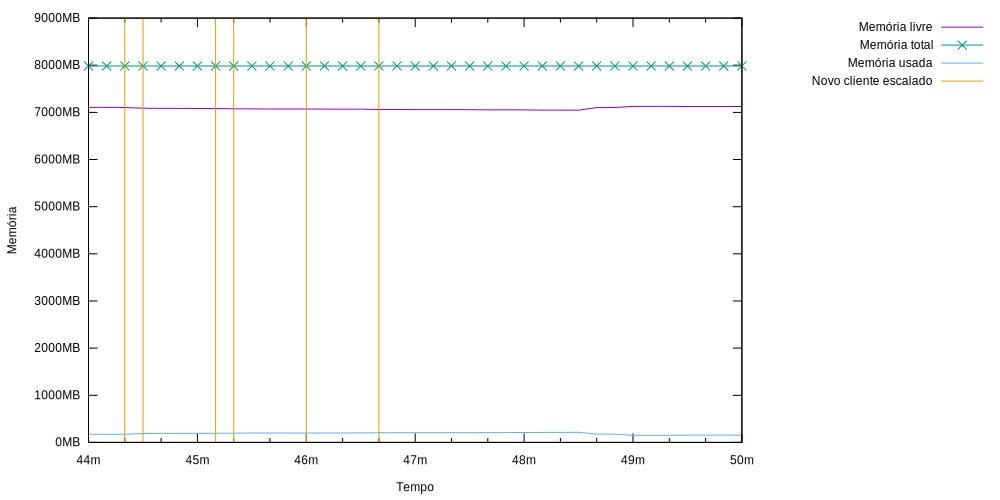
\includegraphics[width=\textwidth]{metricas_rudy_t4/memory.png}
    \centering
    
    Fonte: O próprio autor
\end{figure}

A comparação exibida na Figura~\ref{fig:rudy_t4_memory} mostra somente a escala entre a memória total do serviço com relação a memória consumida.
%
Porém, esta visualização fica comprometida, visto que não fica perceptível a baixa variação da memória consumida com relação ao número de conexões no serviço.
%
A Figura~\ref{fig:rudy_t4_memory_used} trata a escala e aplica somente os dados da memória utilizada pela arquitetura.

\begin{figure}[htb!]
    \caption{Memória consumida no servidor utilizando a arquitetura Rudy}
    \label{fig:rudy_t4_memory_used}
    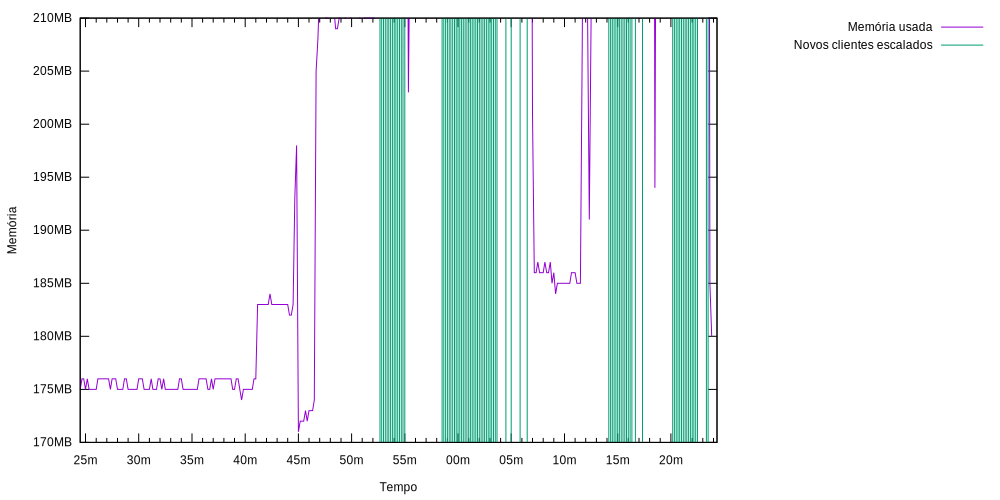
\includegraphics[width=\textwidth]{metricas_rudy_t4/memory_used.png}
    \centering
    
    Fonte: O próprio autor
\end{figure}

Após o tratamento, torna-se notório o crescimento da memória conforme o número de conexões, utilizando uma alícoda de valor pequeno, se comparado ao recurso disponível.
%
Nesse sentido, não foi possível estressar a memória do serviço como um recurso crítico para os testes, porém isto não invalida estes dados para futura comparação com as demais arquiteturas.

\subsection{Consumo de Banda pelo serviço Rudy}

O principal objetivo do monitoramento do consumo da banda pelo serviço Rudy é verificar se a rede está enfileirando as requisições nos serviços \ac{rpc} na arquitetura.
%
Esta validação é feita caso a rede tenha um limite notório na entrada e saída da rede e o aumento do tempo de requisição, sem comprometer a \ac{cpu} do serviço.

Caso as requisições sejam enfileiradas internamente pelo microsserviço \ac{rpc} (Gerente de Jogo), como o modelo de processamento de requisições da arquitetura Rudy propõe, espera-se que o tempo de resposta que aumente.
%
O aumento do tempo de resposta é um reflexo da concorrência para escrever a requisição \ac{rpc} na fila de processamento do serviço, a qual dependerá do escalonador de threads escolher qual processo escreverá a sua requisição na fila.

Com os dados da banda da arquitetura Rudy obtidos do teste, pode-se observar que o crescimento do consumo da rede não é linear.
%
Os dados podem ser visualizados na Figura~\ref{fig:rudy_t4_io}.

\begin{figure}[htb!]
    \caption{Consumo de Banda no servidor utilizando a arquitetura Rudy}
    \label{fig:rudy_t4_io}
    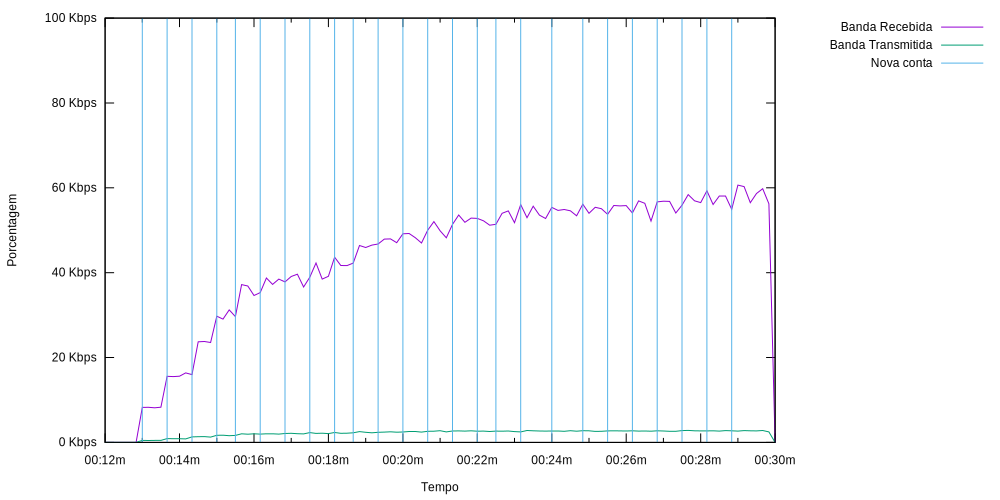
\includegraphics[width=\textwidth]{metricas_rudy_t4/io.png}
    \centering
    
    Fonte: O próprio autor
\end{figure}

Como observado na Figura~\ref{fig:rudy_t4_io}, existe um limite de crescimento da banda.
%
Com as configurações do ambiente, este valor tende a 60Mbps.
%
Vale ressaltar que este gargalo não é proveniente da rede (a qual ficou limitada em 100Mbps), visto que a métrica de latência ficou constante durante os testes.
%
Dessa forma, esta tendência pode ser pela concorrência a fila de processamento, a qual espera-se confirmar com o tempo de resposta do cliente.

\subsection{Tempo de Resposta pelo cliente Rudy}

Para a arquitetura Rudy, o tempo de resposta do cliente irá confirmar se o enfileiramento das requisições \ac{rpc} ocorreram como previsto.
%
Nesse sentido, espera-se que o tempo de requisição aumente de forma superlinear conforme o número de clientes escalados aumente.


Além disso, será possível visualizar o impácto de operações realizadas no banco com o tempo de resposta do serviço, visto que ao efetuar uma operação no banco a mensagem será transmitida pelos microsserviços web dinâmico e pelo gestor do banco de dados, além do banco de dados por fim.
%
Este impácto chamadas sobre o protocolo \ac{http} com múltiplas camadas deve ser notório conforme a demanda de usuários, atrapalhando o gestor de rede com o consumo de \ac{cpu} e rede para atende-los.

Para comparação entre as requisições \ac{rpc} e web, a Figura~\ref{fig:rudy_t4_reqs} exibe ambas em uma única Figura.
%
Espera-se mostrar o crescimento superlinear das requisições \ac{rpc}, a qual chegam a ultrapassar o tempo de resposta das requisições \ac{http} com múltiplas camadas.

\begin{figure}[htb!]
    \caption{Tempo de Resposta do cliente servidor utilizando a arquitetura Rudy}
    \label{fig:rudy_t4_reqs}
    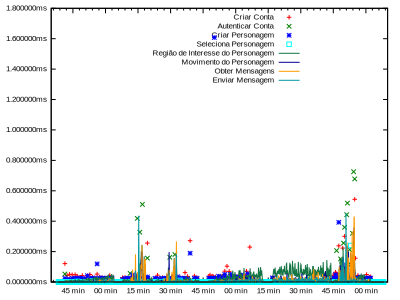
\includegraphics[width=\textwidth]{metricas_rudy_t4/rudyc.png}
    \centering
    
    Fonte: O próprio autor
\end{figure}

A Figura~\ref{fig:rudy_t4_reqs} mostra, dentro de um intervalo de tempo, o tempo de resposta categorizado conforme a ação realizada pelo cliente no serviço.
%
Para facilitar a visualização, este gráfico foi dividido em duas categorias, segregando as requisições sobre \ac{http} e sobre \ac{rpc}.
%
A Figura~\ref{fig:rudy_t4_reqs_https} exibe o tempo de resposta das requisições web em relação ao tempo.
%
Mostra-se na figura a dispersão que ocorre nos tempos de requisições sobre o protocolo \ac{http} conforme o recurso do serviço é consumido por novos clientes.
 

\begin{figure}[htb!]
    \caption{Tempo de Resposta de requisições \textit{Web} do cliente servidor utilizando a arquitetura Rudy}
    \label{fig:rudy_t4_reqs_https}
    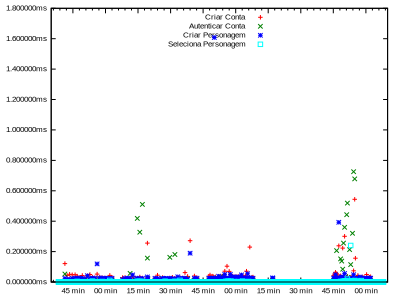
\includegraphics[width=\textwidth]{metricas_rudy_t4/rudyc_http.png}
    \centering
    
    Fonte: O próprio autor
\end{figure}

A Figura~\ref{fig:rudy_t4_reqs_https} exibe uma dispersão conforme o número de conexões do serviço aumenta.
%
Entretanto, espera-se que este tempo de requisição sobre o protocolo \ac{http} aumente somente como um reflexo do consumo de \ac{cpu} e banda pelos clientes.
%
Por este motivo, é notório a necessidade de exibir a parte o tempo de requisição das chamadas \ac{rpc}.
%
Os dados do protocolo \ac{rpc} podem ser visualizados na Figura~\ref{fig:rudy_t4_reqs_rpc}.

\begin{figure}[htb!]
    \caption{Tempo de Resposta de requisições \ac{rpc} do cliente servidor utilizando a arquitetura Rudy}
    \label{fig:rudy_t4_reqs_rpc}
    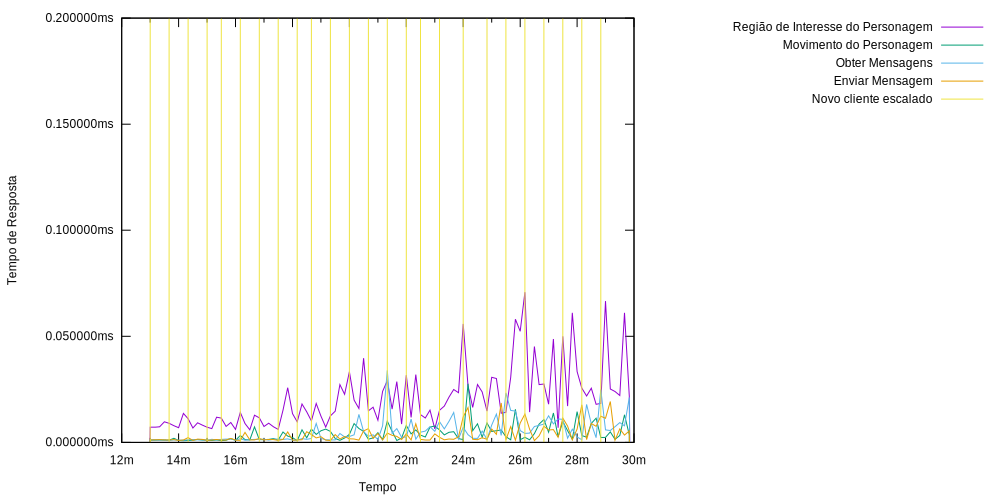
\includegraphics[width=\textwidth]{metricas_rudy_t4/rudyc_rpc.png}
    \centering
    
    Fonte: O próprio autor
\end{figure}

A Figura~\ref{fig:rudy_t4_reqs_rpc} exibe o desparelhamento provocado pelo sistema de filas implementado nesta arquitetura nos serviços \ac{rpc}.
%
Percebe-se também que esta disparidade aumenta diretamente com as requisições \ac{http} ao escalar um novo cliente.
%
Estas informações indicam que de fato ocorre o enfileiramento das requisições, além disso a carga das requisições \ac{http} agravam o enfileiramento, aumentando significantemente o tempo de resposta durante os próximos segundos após a chamada \ac{http}.

A partir dos dados obtidos das requisições \ac{http}, exibidos na Figura~\ref{fig:rudy_t4_reqs_https}, percebe-se que os valores exercem baixa influência conforme a carga de usuários utilizando o serviço.
%
Nesse sentido, é possível agrupar todos os dados a fim de obter a sua média, mediana, valor máximo e mínimo das requisições sobre o protocolo \ac{http}.
%
Estes dados estão dispostos na Tabela~\ref{tab:medias_http_rudy}.

\begin{table}[htb!]
    \centering
    \caption{Média, mediana, máximo e mínimo obtidos pelas requisições HTTP.}
    \label{tab:medias_http_rudy}
    \begin{adjustbox}{width=1\textwidth}
    \begin{tabular}{|l|l|l|l|l|}
    \hline
    Requisição HTTP       & Máximo      & Mínimo        & Média            & Mediana          \\ \hline
    Criar conta           & 0,221395227 s & 0,020872847 s & 0,039408472375 s & 0,0292280260 s \\ \hline
    Autenticar Conta      & 0,207815276 s & 0,007954407 s & 0,019106303125 s & 0,0106579220 s \\ \hline
    Criar Personagem      & 0,090555727 s & 0,019188871 s & 0,027868142025 s & 0,0250552605 s \\ \hline
    Selecionar Personagem & 0,010201612 s & 0,000752974 s & 0,002188604100 s & 0,0021886041 s \\ \hline
    \end{tabular}
    \end{adjustbox}

    Fonte: O próprio autor.
\end{table}

A Tabela~\ref{tab:medias_http_rudy} comprova a estabilidade das requisições \ac{http}, na qual a média, mediana e o valor mínimo estão próximos para todos os tipos de requisição.
%
Nota-se pela Requisição \ac{http} Selecionar Personagem, na qual realiza a busca dos dados no banco em parapelo a requisição, a maior estabilidade e eficiência dentre as demais citadas.
%
Nesse sentido, torna-se visível que a instabilidade, por mais que baixa, esteja relacionada com a busca ou inserção de dados nos bancos da arquitetura.

As requisições \ac{rpc} também podem apresentar caracteristicas similares.
%
Entretanto, as requisições \ac{rpc} concorrem com as requisições \ac{http} entre os recursos do serviço.
%
Nesse sentido, torna-se interessante obter a média, mediana, máximo e mínimo dos tempos de requisição levando em consideração o número de clientes escalados.
%
A Tabela~\ref{tab:medias_rpc_rudy} exibe a média, mediana, máximo e mínimo, segregando conforme o número de conexões do serviço.